\documentclass{beamer}
\usepackage{epstopdf}
\usepackage{amssymb,amsmath}
\usepackage{hyperref}
\usepackage{verbatim}
\definecolor{links}{HTML}{2A1B81} 
\hypersetup{colorlinks,linkcolor=,urlcolor=links}
%\usepackage{xcolor}
\usepackage{pgfplots}
\usepackage{tikz}
%\usepackage[usenames,dvipsnames]{color}
\usetikzlibrary{arrows,shapes,positioning}
\definecolor{BrickRed}{RGB}{178,34,34}
\definecolor{Navy}{RGB}{0,0,128}
\definecolor{Teal}{RGB}{0,128,128}
\definecolor{Green}{RGB}{0,128,0}



\usepackage{graphicx}
\usepackage{multirow}
\usepackage[overlay]{textpos}
\usetheme{Copenhagen}
\usecolortheme{beaver}
\usecolortheme{orchid}
\setbeamertemplate{navigation symbols}{\insertframenumber} 
\colorlet{lightgray}{gray!40}
\setbeamercolor{postit}{fg=purple,bg=lightgray}
% \usepackage{beamerthemesplit} // Activate for custom appearance


\addtobeamertemplate{frametitle}{}{%
\begin{textblock*}{50mm}(.92\textwidth,-0.8cm)
\includegraphics[height=0.55cm,width=1.5cm]{/Users/caitlinmalone/Documents/ATLAS/slac_logo.pdf}
\end{textblock*}}

% \usepackage{beamerthemesplit} // Activate for custom appearance

\title{Higgs Bosons Decaying to Fermions in ATLAS and CMS}
%\subtitle{Higgs Couplings 2013, Freiburg}
\author{Caitlin Malone, SLAC}
\institute{on behalf of the ATLAS Collaboration\\Higgs Couplings 2013, Freiburg\\14 October 2013 }
\date{}

\begin{document}

\frame{\titlepage}


\begin{frame}{Introduction}
	\begin{itemize} \scriptsize
		\item New Higgs boson discovered near 125 GeV first seen and studied in bosonic channels \textcolor{Teal}{($H\rightarrow\gamma\gamma$, $H\rightarrow ZZ\rightarrow 4l$, $H\rightarrow WW \rightarrow l\nu l \nu$)}
		\item At a mass of 125 GeV, Higgs boson decays in many channels, including \textcolor{BrickRed}{quarks and leptons $H\rightarrow bb$, $H\rightarrow\tau\tau$, $H\rightarrow\mu\mu$}
	\end{itemize}
	\begin{columns}[c]
		\column{0.6\textwidth}
			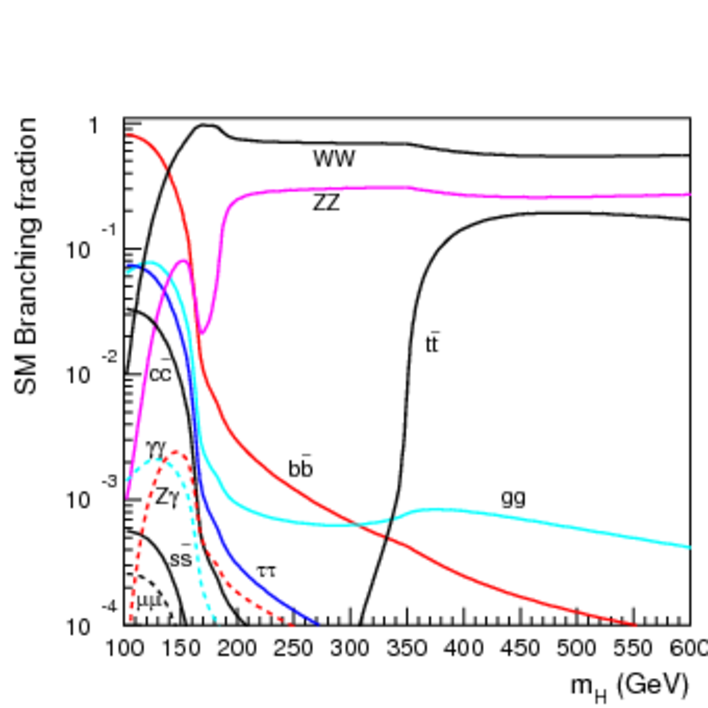
\includegraphics[width=\textwidth]{/Users/caitlinmalone/Documents/ATLAS/HiggsCouplings2013/figures/h_br_sm.pdf}
		\column{0.4\textwidth}
	\end{columns}

\end{frame}


\begin{frame}{Production Channels}
	\begin{columns}[c]
	\column{0.25\textwidth}
		\scriptsize \textcolor{BrickRed}{gluon fusion:} \\
		- $\sigma\approx$ 15 pb \\
		- can get additional jets or high-$p_T$ Higgs \\
		- top quark loop provides main constraint on Higgs couplings to quarks
		\vspace{1cm}
		
		\textcolor{BrickRed}{W/Z associated production:} \\
		- $\sigma\approx$0.58 (W) or 0.34 (Z) pb \\
		- vector boson allows easier triggering and tagging
		
	\column{0.5\textwidth}
		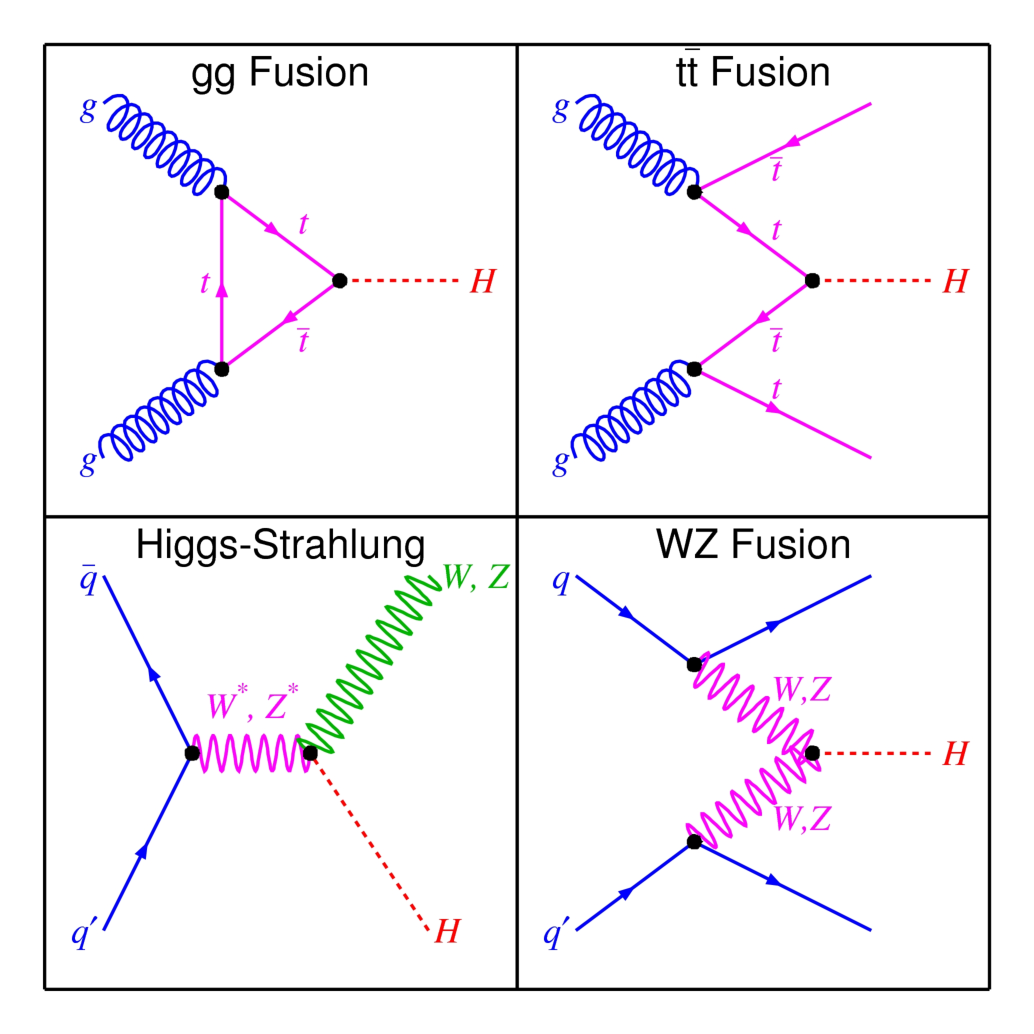
\includegraphics[width=\textwidth]{/Users/caitlinmalone/Documents/ATLAS/HiggsCouplings2013/figures/higgs_feyn_pp.pdf}
		
		
	\column{0.25\textwidth}
		\scriptsize \textcolor{BrickRed}{ttH:}\\
		- $\sigma\approx$ 0.086 pb\\
		- top quarks allow easier triggering and tagging
		
		\vspace{2cm}
		
		\textcolor{BrickRed}{Vector Boson Fusion:} \\
		- $\sigma\approx$1.2 pb \\
		- forward jets provide unique signature		
	\end{columns}
\end{frame}






\begin{frame}[c]
	\frametitle{\ }
	\begin{center}
	\huge \textcolor{Navy}{$H\rightarrow\tau\tau$}
	\end{center}
\end{frame}



\begin{frame}{$H\rightarrow \tau \tau$ Motivation}
	\begin{columns}[c]
	\column{0.6\textwidth}
	\begin{itemize} \scriptsize

		\item \textcolor{BrickRed}{Direct coupling to lepton sector}
		\item 4th channel for observation, after vector bosons and $\gamma \gamma$
		\item \textcolor{BrickRed}{6.3\% branching ratio at $m_H$=125 GeV}
		\item \textcolor{Navy}{Analyses categorized by decay mode, to allow optimization to different backgrounds}

	\end{itemize}
	\column{0.4\textwidth}
		\includegraphics[width=\textwidth]{figures/tau_decay.pdf}
	\end{columns}
	
	\vspace{1cm}

	\begin{columns}
		\column{0.33\textwidth}
			$\tau_{lep}\tau_{lep}$
			\begin{itemize} \scriptsize
				\item lep=$\mu, e$
				\item \textcolor{Navy}{cleanest channel}
				\item $\mu$ generally cleaner than $e$ in detector, lower backgrounds
				\item \textcolor{BrickRed}{price: 12\% branching fraction, Drell-Yan backgrounds}
			\end{itemize}

		\column{0.33\textwidth}
			$\tau_{had}\tau_{had}$
			\begin{itemize} \scriptsize
				\item \textcolor{Navy}{42\% branching ratio, small Drell-Yan background}
				\item \textcolor{BrickRed}{price: larger QCD jets background, jet energy scale/resolution}
			\end{itemize}

		\column{0.33\textwidth}

			$\tau_{lep}\tau_{had}$

				\begin{itemize}	\scriptsize		
					\item \textcolor{Navy}{best of both worlds: clean lepton tag, 46\% branching ratio}
					\item \textcolor{BrickRed}{generally channel with most power}
				\end{itemize}
	\end{columns}
\end{frame}




\begin{frame}{$H \rightarrow \tau \tau$: Overview of Analyses}
	\begin{table}
%		\scriptsize
		\begin{tabular}{c | c | c | c | c | c | c}
		
		
		 & VBF & Boosted & VH & 1-jet$^*$ & ttH & 0-jet$^{**}$\\ \hline \hline
		 
				
			$\mu \tau_{had}$ &
			
\includegraphics[width=0.05\textwidth]{figures/atlas_logo.pdf} 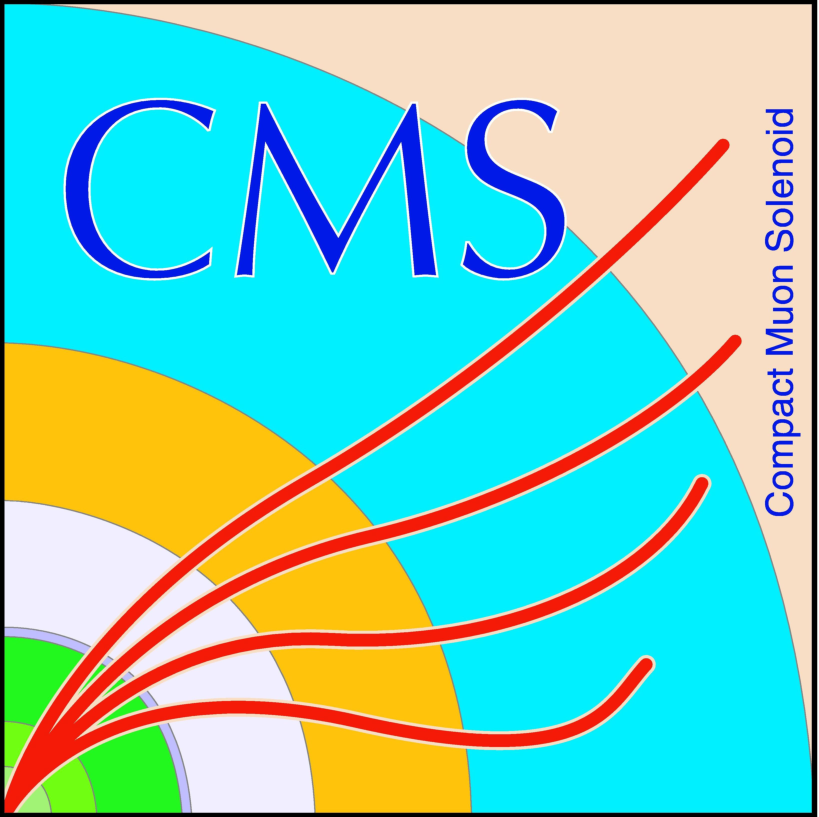
\includegraphics[width=0.05\textwidth]{figures/cms_logo.pdf} &
			
\includegraphics[width=0.05\textwidth]{figures/atlas_logo.pdf} &
			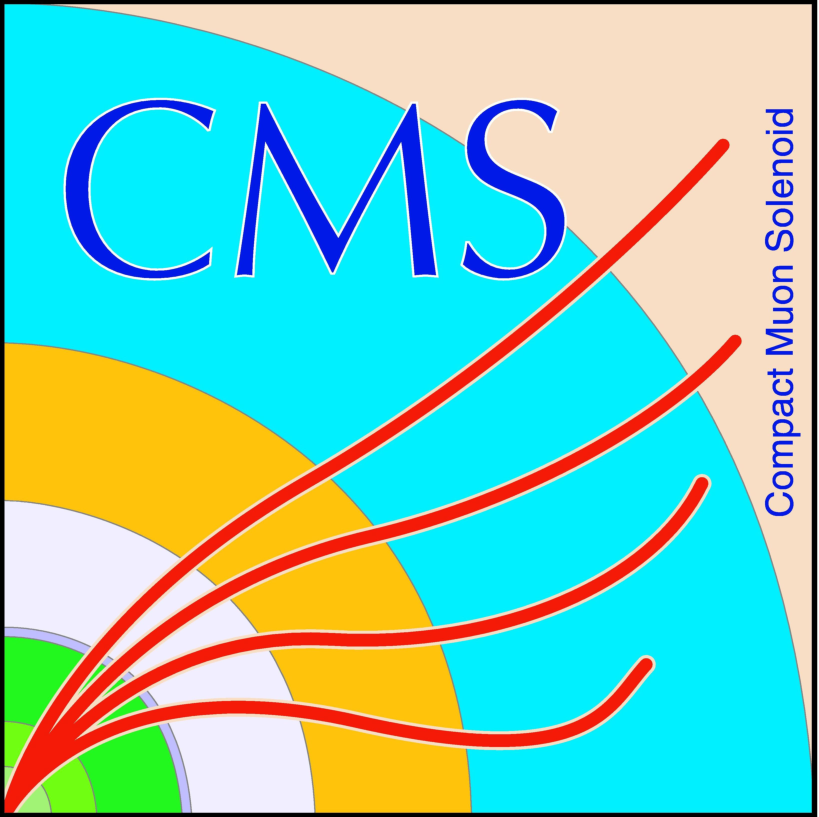
\includegraphics[width=0.05\textwidth]{figures/cms_logo.pdf}&

			
\includegraphics[width=0.05\textwidth]{figures/atlas_logo.pdf} 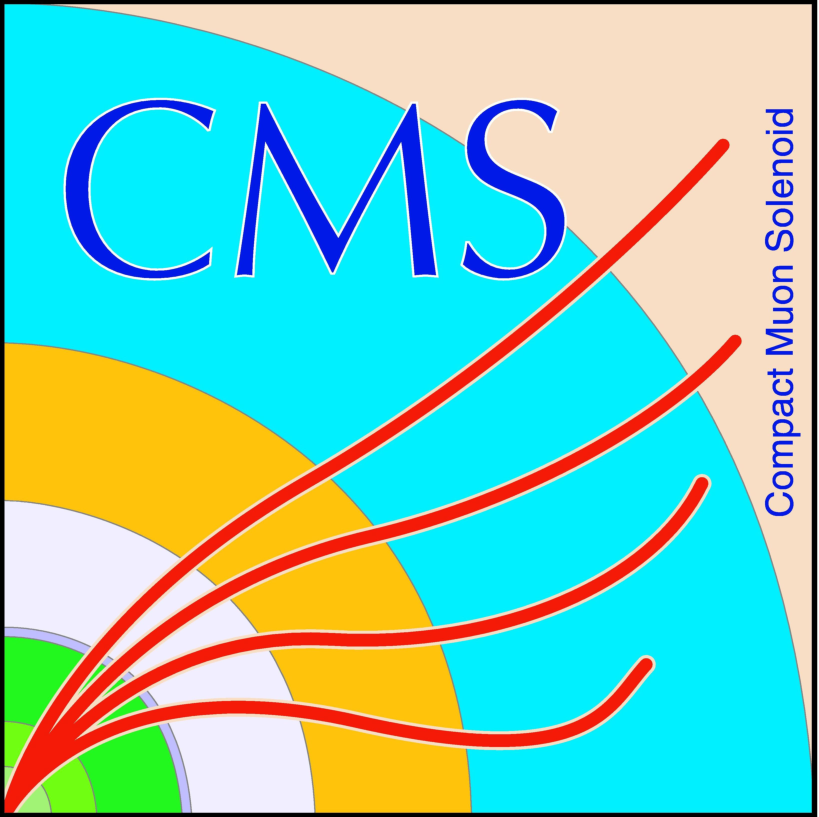
\includegraphics[width=0.05\textwidth]{figures/cms_logo.pdf} &
			&
			
\includegraphics[width=0.05\textwidth]{figures/atlas_logo.pdf} 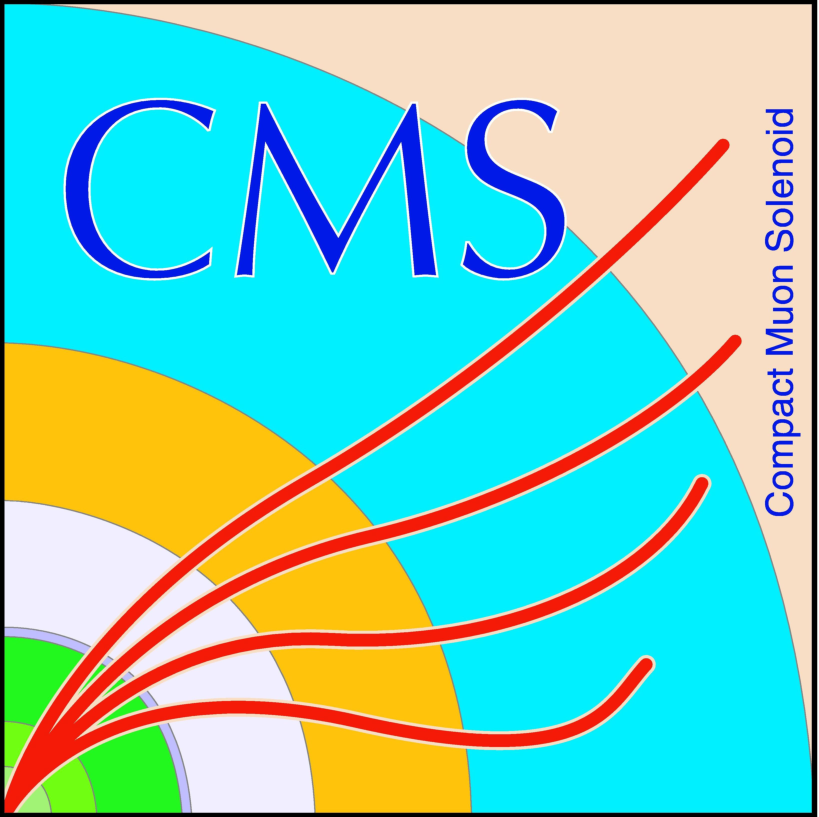
\includegraphics[width=0.05\textwidth]{figures/cms_logo.pdf} 	
			\\	
			$e \tau_{had}$ &
			
\includegraphics[width=0.05\textwidth]{figures/atlas_logo.pdf} 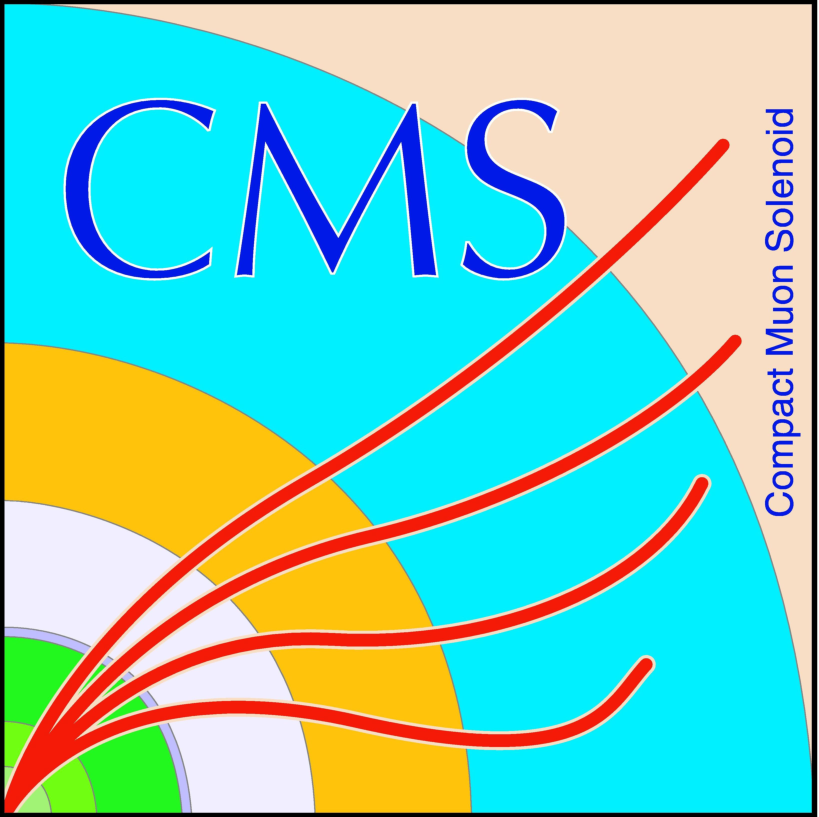
\includegraphics[width=0.05\textwidth]{figures/cms_logo.pdf} &
			
\includegraphics[width=0.05\textwidth]{figures/atlas_logo.pdf} &
			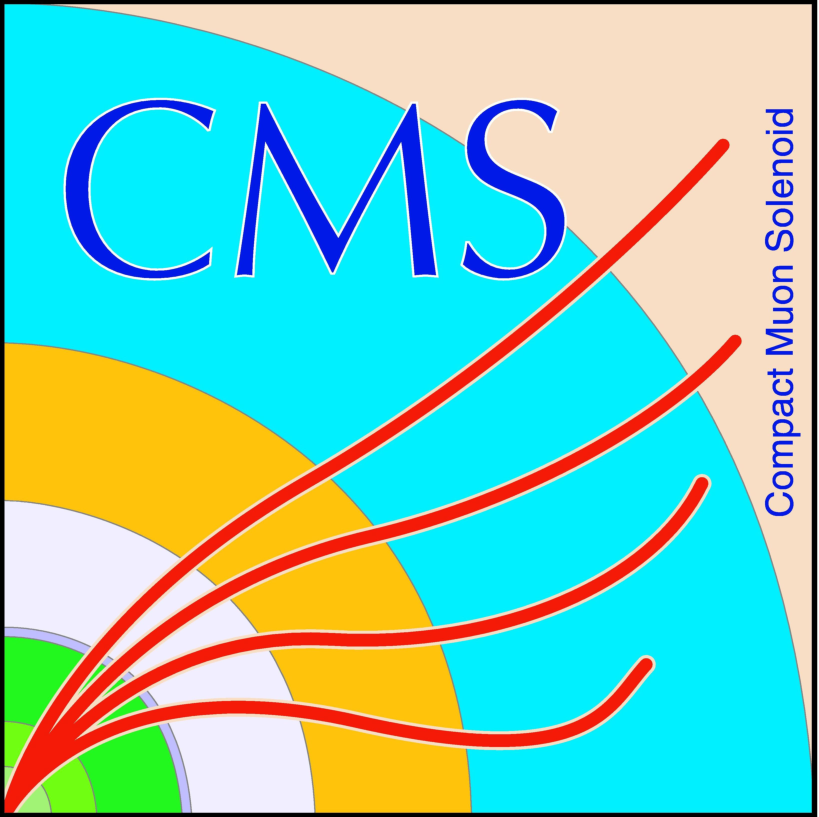
\includegraphics[width=0.05\textwidth]{figures/cms_logo.pdf} &
			
\includegraphics[width=0.05\textwidth]{figures/atlas_logo.pdf} 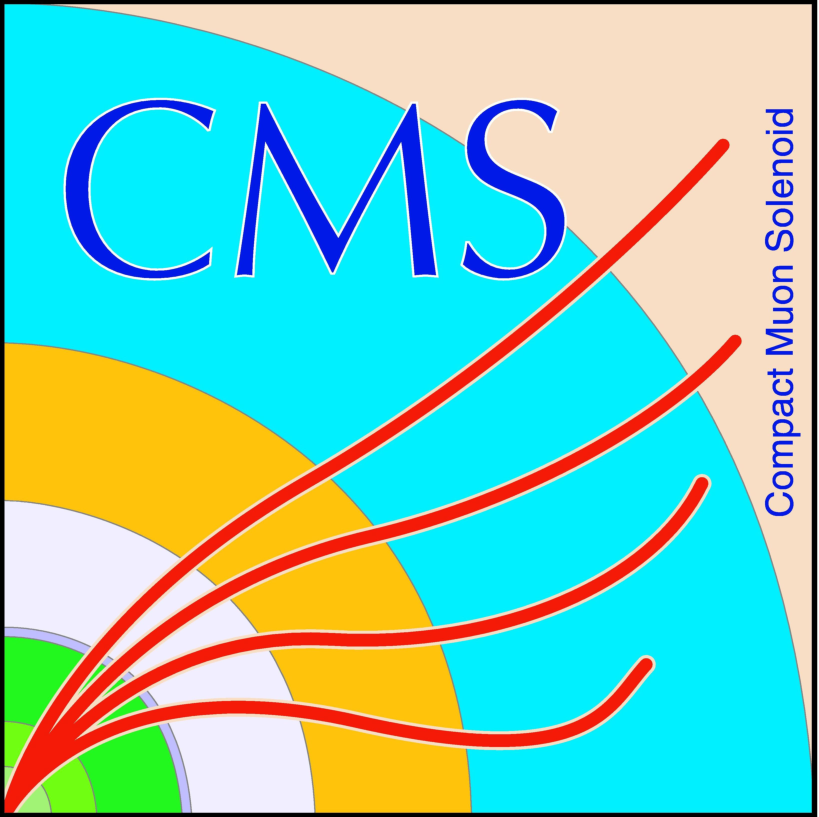
\includegraphics[width=0.05\textwidth]{figures/cms_logo.pdf} &
			&
			
\includegraphics[width=0.05\textwidth]{figures/atlas_logo.pdf} 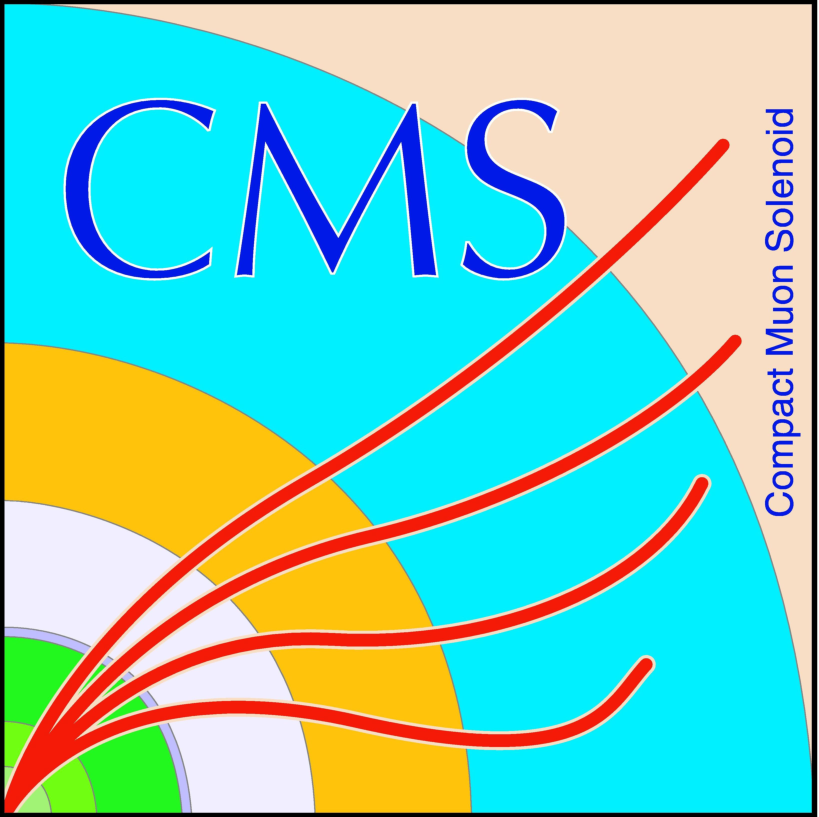
\includegraphics[width=0.05\textwidth]{figures/cms_logo.pdf} 	
			\\	
			
			 
			\hline		
			$\mu e$ &
			
\includegraphics[width=0.05\textwidth]{figures/atlas_logo.pdf} 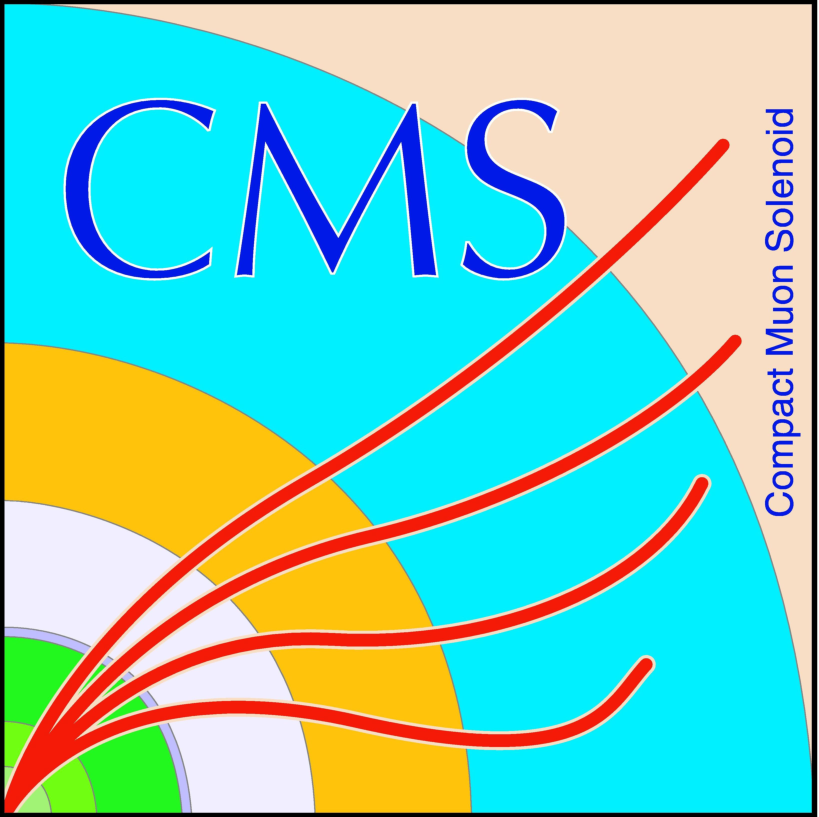
\includegraphics[width=0.05\textwidth]{figures/cms_logo.pdf} &
			
\includegraphics[width=0.05\textwidth]{figures/atlas_logo.pdf} &
			
\includegraphics[width=0.05\textwidth]{figures/atlas_logo.pdf} 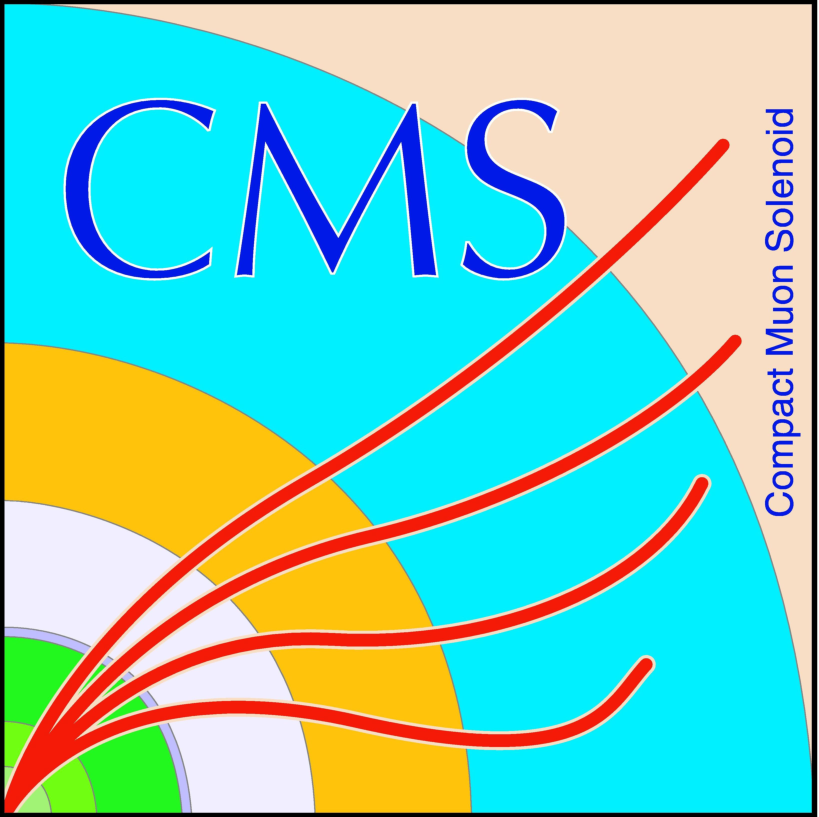
\includegraphics[width=0.05\textwidth]{figures/cms_logo.pdf}&
			
\includegraphics[width=0.05\textwidth]{figures/atlas_logo.pdf} 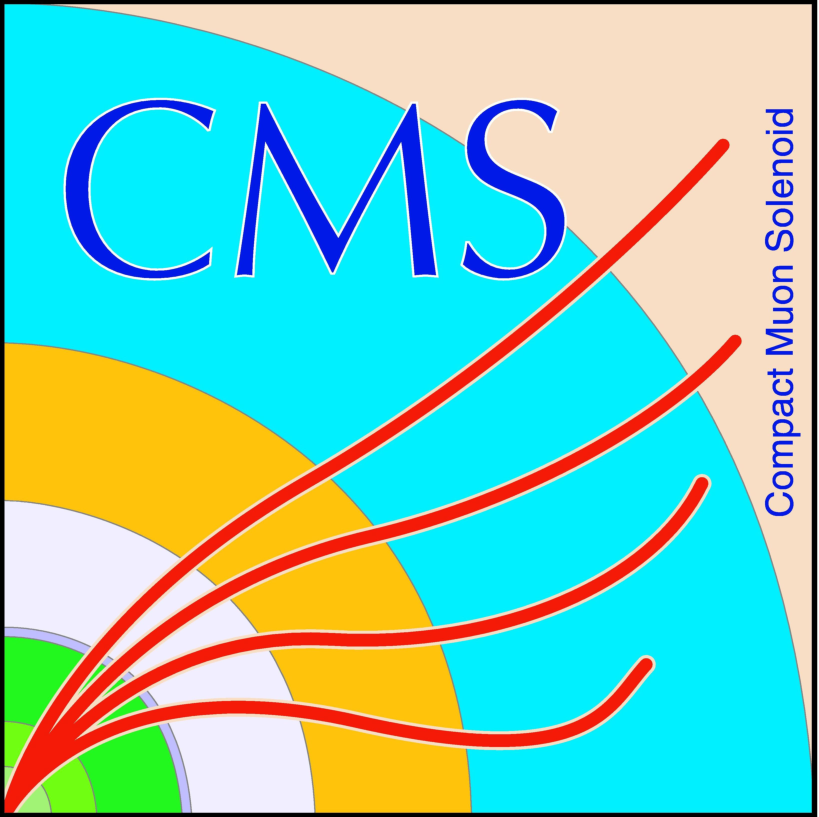
\includegraphics[width=0.05\textwidth]{figures/cms_logo.pdf} &
			&
			
\includegraphics[width=0.05\textwidth]{figures/atlas_logo.pdf} 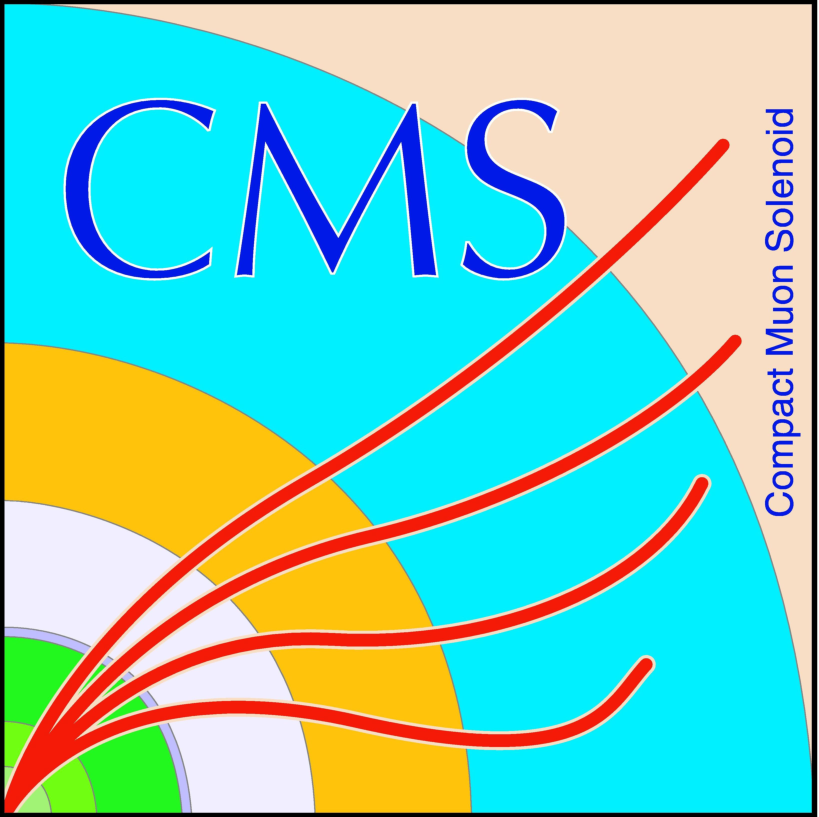
\includegraphics[width=0.05\textwidth]{figures/cms_logo.pdf} 	
			\\
			$\mu\mu$ &
			
\includegraphics[width=0.05\textwidth]{figures/atlas_logo.pdf} 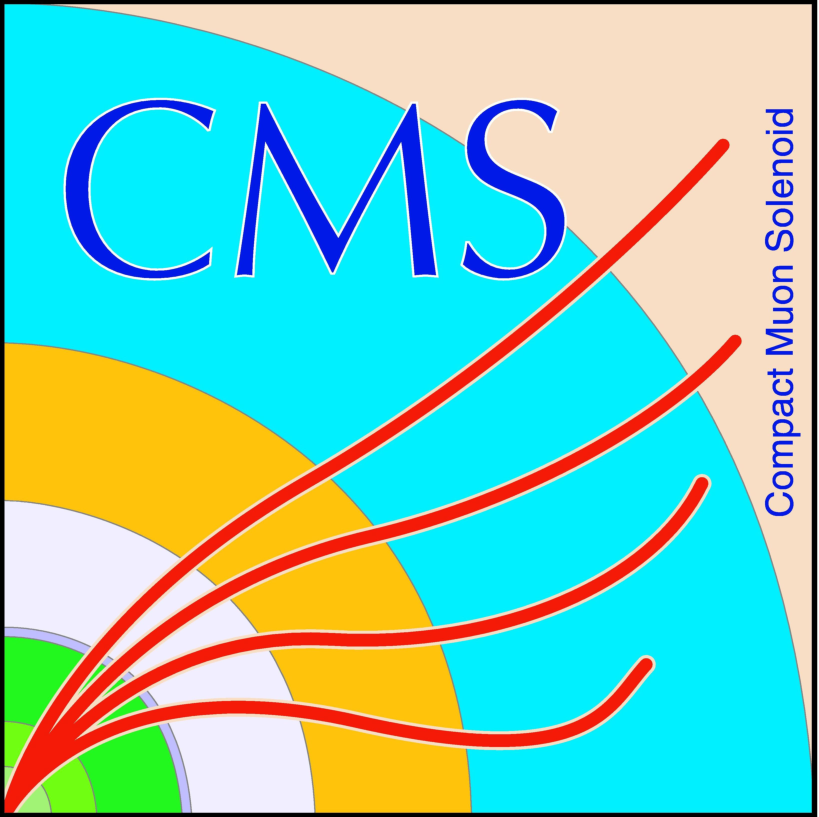
\includegraphics[width=0.05\textwidth]{figures/cms_logo.pdf} &
			
\includegraphics[width=0.05\textwidth]{figures/atlas_logo.pdf} &
			
\includegraphics[width=0.05\textwidth]{figures/atlas_logo.pdf} &
			
\includegraphics[width=0.05\textwidth]{figures/atlas_logo.pdf} 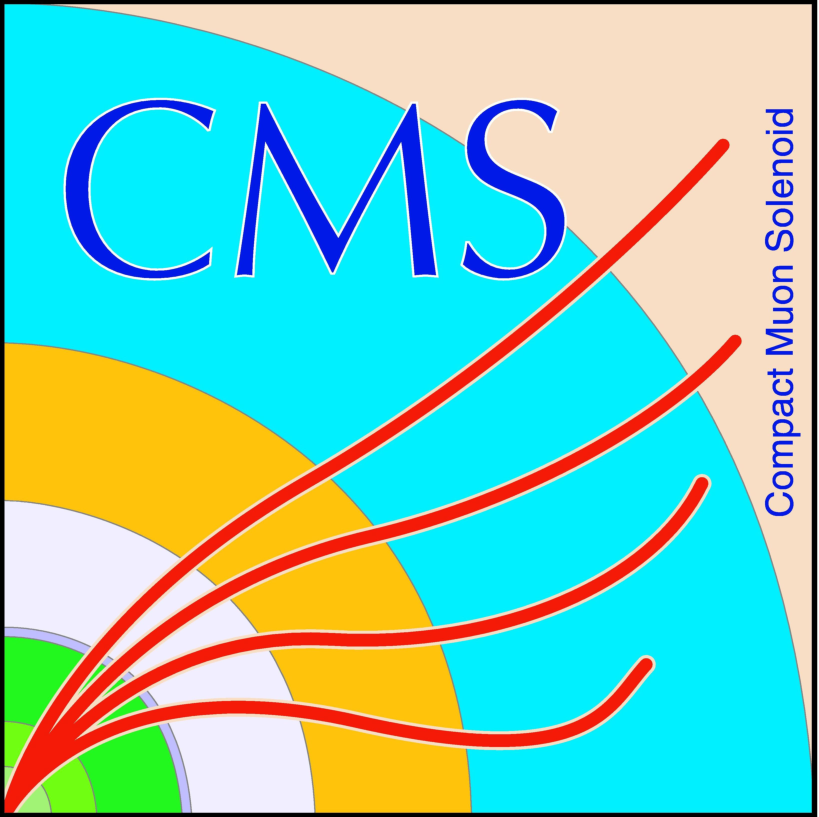
\includegraphics[width=0.05\textwidth]{figures/cms_logo.pdf} &
			&
			
\includegraphics[width=0.05\textwidth]{figures/atlas_logo.pdf} 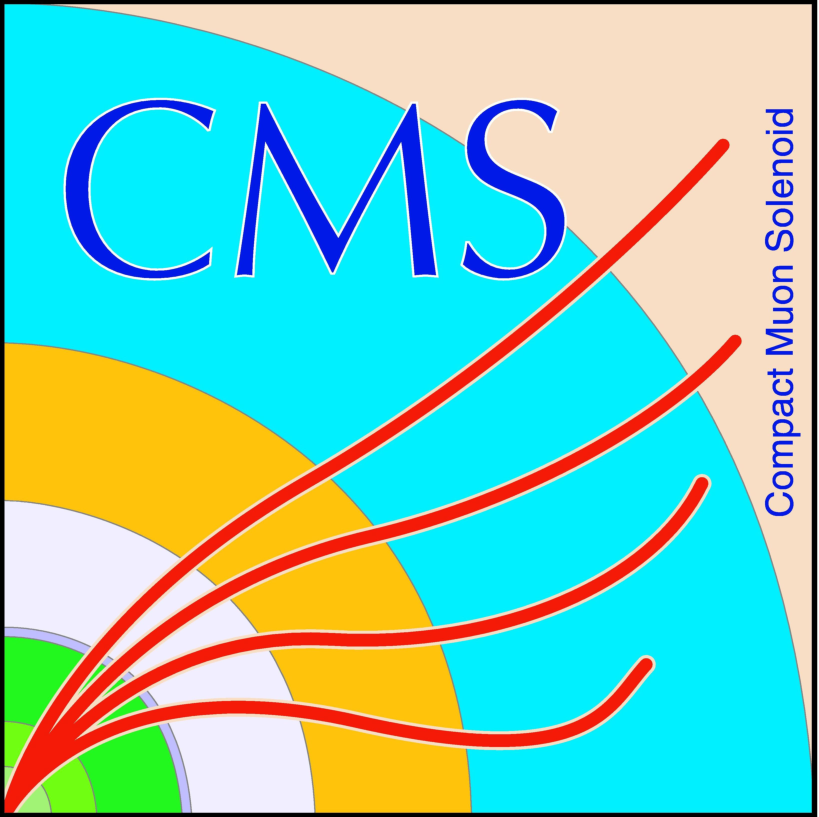
\includegraphics[width=0.05\textwidth]{figures/cms_logo.pdf} 	
			\\
			$ee$ &
			
\includegraphics[width=0.05\textwidth]{figures/atlas_logo.pdf} &
			
\includegraphics[width=0.05\textwidth]{figures/atlas_logo.pdf} &
			
\includegraphics[width=0.05\textwidth]{figures/atlas_logo.pdf} &
			
\includegraphics[width=0.05\textwidth]{figures/atlas_logo.pdf} &
			&
			
\includegraphics[width=0.05\textwidth]{figures/atlas_logo.pdf} 	
			\\	


			
			\hline
			$\tau_{had} \tau_{had}$ &
			
\includegraphics[width=0.05\textwidth]{figures/atlas_logo.pdf} 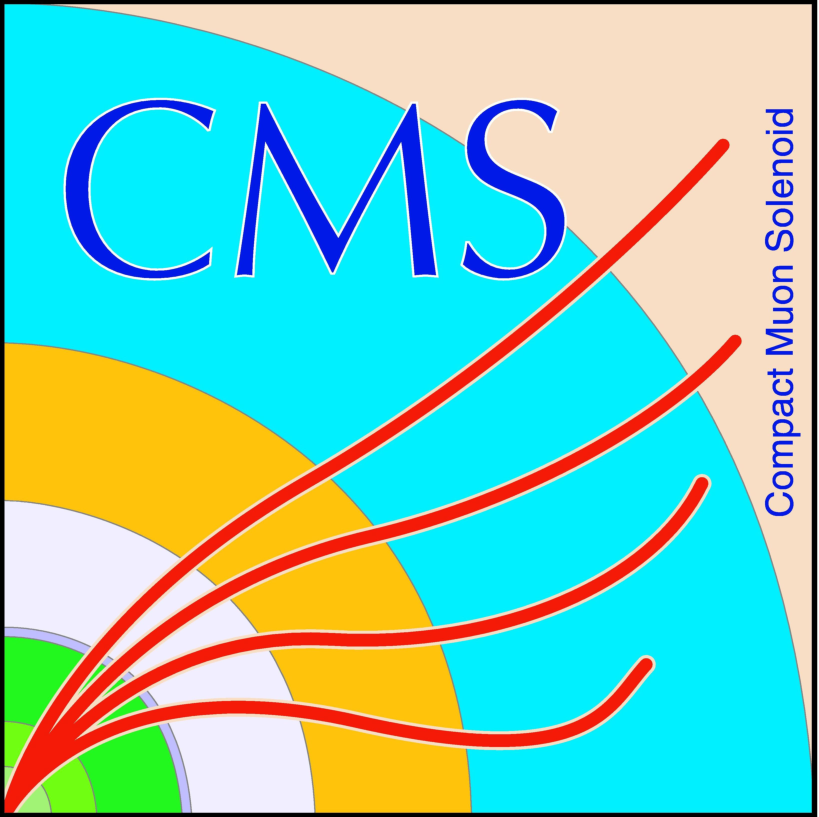
\includegraphics[width=0.05\textwidth]{figures/cms_logo.pdf} &
			
\includegraphics[width=0.05\textwidth]{figures/atlas_logo.pdf} 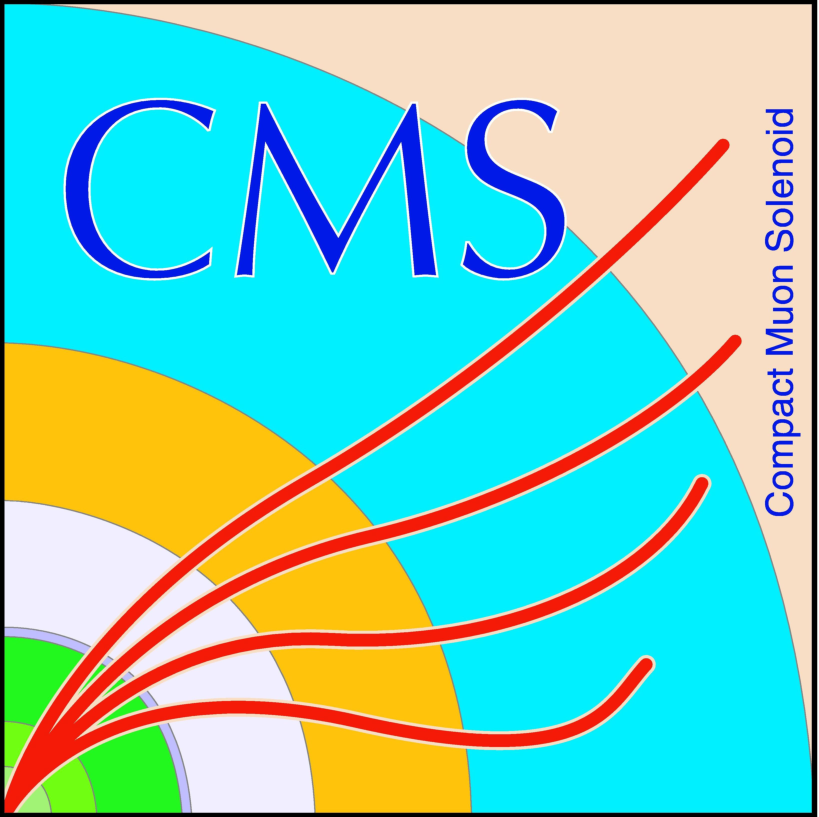
\includegraphics[width=0.05\textwidth]{figures/cms_logo.pdf} &	
			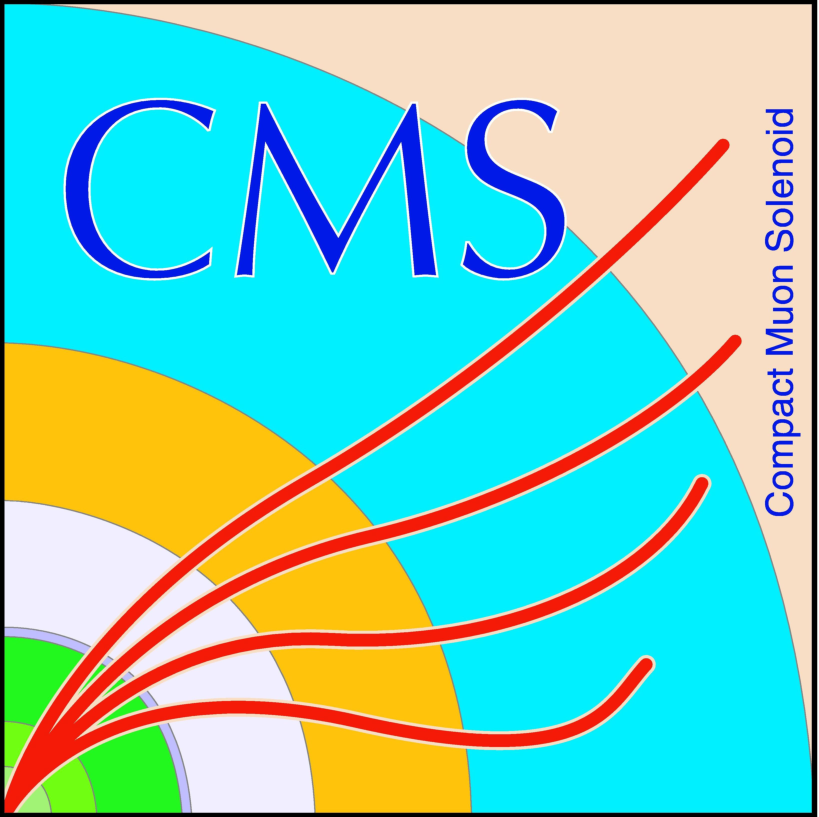
\includegraphics[width=0.05\textwidth]{figures/cms_logo.pdf}&
			&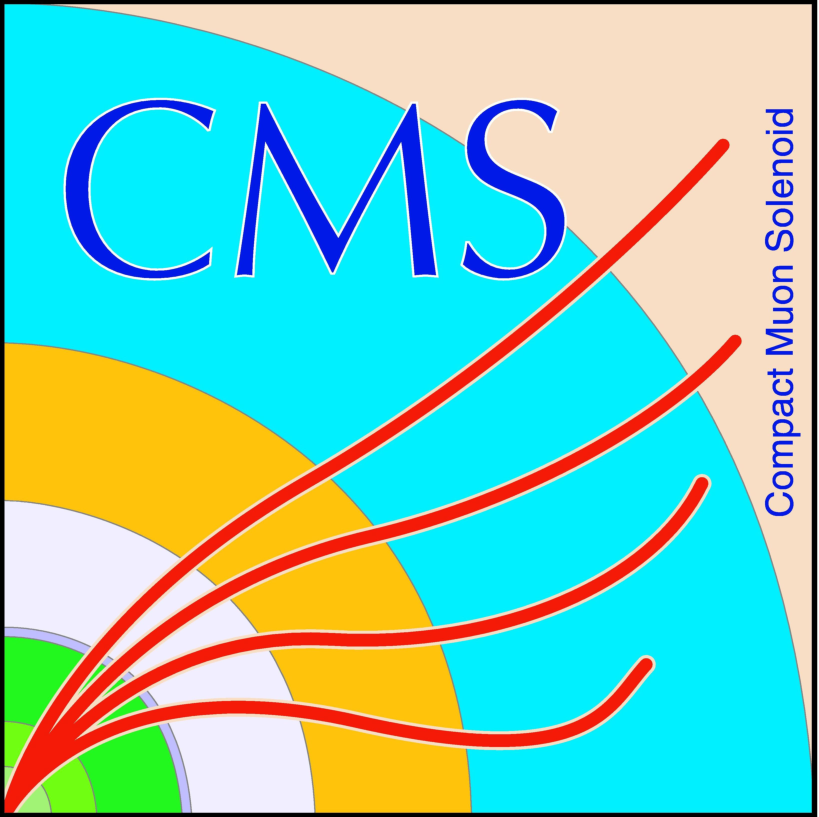
\includegraphics[width=0.05\textwidth]{figures/cms_logo.pdf} 
			&  
			\\					
				
		\end{tabular}
	\end{table}
	\scriptsize
	\textcolor{BrickRed}{$^{*}$ CMS splits 1-jet category based on $p_T$ of lepton or $\tau$} \newline
	\textcolor{BrickRed}{$^{**}$ ATLAS: 7 TeV only; CMS: control region only} \\
	NB: Analysis definitions not identical between collaborations!  See notes for more detail
\end{frame}



\begin{frame}{$\tau$ Reconstruction and Embedding}

\end{frame}



\begin{frame}{CMS Analysis}

\end{frame}






\begin{frame}{CMS $H\rightarrow \tau \tau$: Results}
	\begin{columns}[c]
		\column{0.5\textwidth}
			\includegraphics[width=0.9\textwidth]{/Users/caitlinmalone/Documents/ATLAS/HiggsCouplings2013/figures/cms_htautau_brazil.pdf}\\
		\column{0.5\textwidth}
			\includegraphics[width=0.9\textwidth]{/Users/caitlinmalone/Documents/ATLAS/HiggsCouplings2013/figures/cms_htautau_p_value.pdf}\\
	\end{columns}	
	\vspace{0.5cm}
	\begin{columns}
		\column{0.5\textwidth}
			\scriptsize 
			At $m_H$=125 GeV, observed (expected) 95\% CL upper limit on cross section is 1.0 (1.63) $\times$ SM (background-only hypothesis)
		\column{0.5\textwidth}
			\scriptsize
			For $m_H$=125 GeV, observed (expected) p-value 2.85 (2.62) and best fit value $\mu$=1.1$\pm$0.4 
	\end{columns}	

\end{frame}



\begin{frame}{ATLAS Analysis and MMC}

\end{frame}






\begin{frame}{ATLAS $H\rightarrow\tau\tau$: Results}
	\begin{columns}[c]
		\column{0.5\textwidth}
			\includegraphics[width=\textwidth]{/Users/caitlinmalone/Documents/ATLAS/HiggsCouplings2013/figures/atlas_htautau_brazil.pdf}
		\column{0.5\textwidth}
			\includegraphics[width=\textwidth]{/Users/caitlinmalone/Documents/ATLAS/HiggsCouplings2013/figures/atlas_htautau_p_value.pdf}
	\end{columns}
	
	\begin{columns}[c]
		\column{0.5\textwidth}
			\scriptsize
			For $m_H$=125 GeV, observed (expected) 95\% CL upper limits on cross section is 1.9 (1.2) $\times$ SM (background-only hypothesis)
		\column{0.5\textwidth}
			\scriptsize
			For $m_H$=125 GeV, observed (expected) p-value 1.1 (1.7)$\sigma$ and best fit value $\mu$=0.7$\pm$0.7
	\end{columns}
\end{frame}




\begin{frame}[c]
	\begin{center}
	\huge \textcolor{Navy}{$H\rightarrow bb$}
	\end{center}
\end{frame}



\begin{frame}{$H\rightarrow bb$ Motivation}
		\textcolor{BrickRed}{- Only experimentally visible decay mode to quarks}\\
		- Main way to probe couplings to down-type quarks \\
		\textcolor{Teal}{- Inclusive production (ggF) impossible to observe because of high QCD background}\\
		\textcolor{Navy}{- Require extra particles or a unique topology}\\
		\vspace{0.2cm}
			\scriptsize{
			\hspace{1cm}	- Forward jets: characteristic of VBF topology\\
			\hspace{1cm}	- Top quark pair: \\
			\hspace{1cm}	- Vector bosons: $Z\rightarrow\nu\nu$, $W\rightarrow l\nu$, $Z\rightarrow ll$\\
			}
		\vspace{0.2cm}
		\normalsize
		\textcolor{BrickRed}{- High branching ratio (about 58\%) means that observation is crucial to constrain the overall Higgs width}

\end{frame}


\begin{frame}{CMS VBF $H\rightarrow bb$}	
	\begin{columns}[c]
		\column{0.33\textwidth}	
			\scriptsize Event topology characterized by large $\Delta\eta$ between non-b-tagged jets	
			\includegraphics[width=1.1\textwidth]{/Users/caitlinmalone/Documents/ATLAS/HiggsCouplings2013/figures/cms_vbfhbb_delta_eta.pdf}
		\column{0.33\textwidth}
			\scriptsize ANN discriminant based on event topology and b-tag values
			\includegraphics[width=1.1\textwidth]{/Users/caitlinmalone/Documents/ATLAS/HiggsCouplings2013/figures/cms_vbfhbb_ann_output.pdf}
		\column{0.33\textwidth}
			\scriptsize Highest categories of ANN heavily dominated by VBF production (vs. ggF)
			\includegraphics[width=1.1\textwidth]{/Users/caitlinmalone/Documents/ATLAS/HiggsCouplings2013/figures/cms_vbfhbb_ann_categories.pdf}
	\end{columns}
	\begin{columns}[c]
		\column{0.5\textwidth}
			\includegraphics[width=\textwidth]{/Users/caitlinmalone/Documents/ATLAS/HiggsCouplings2013/figures/cms_vbfhbb_brazil.pdf}
		\column{0.5\textwidth}
		\scriptsize 

		For $m_H$=125 GeV, 95\% CL upper limits on cross section is 3.6 (3.0) $\times$ SM (background-only hypothesis) and observed signal strength $\mu$=0.7$\pm$1.4
	\end{columns}
	\scriptsize\textcolor{Teal}{ATLAS VBF results still in progress, with result planned for winter 2014}
\end{frame}



\begin{frame}{CMS ttH}

\end{frame}


\begin{frame}{ATLAS ttH}

\end{frame}








\begin{frame}{Binning in $P^V_T$}
	\scriptsize
	\textcolor{Teal}{Backgrounds are substantially reduced by requiring a significant boost of the $p_T$ of the vector boson, $p^V_T$. \\}
	\textcolor{Navy}{The boost categories (all numbers in GeV) below are for CMS and ATLAS.}
	\begin{columns}[c]
		\column{0.5\textwidth}
			\begin{table}
			\scriptsize
			\begin{tabular}{c | c | c | c }
				& low & medium & high \\ \hline
			W($l\nu$) & 100-130 & 130-180 & $>$180 \\
			W($\tau\nu$) & & & $>$120 \\
			Z($\nu\nu$)  & 100-130 & 130-170 & $>$170 \\
			Z($ll$)   & 50-100 & & $>$100 \\
			\end{tabular}
			\end{table}
		\column{0.5\textwidth}
	\includegraphics[width=0.25\textwidth]{/Users/caitlinmalone/Documents/ATLAS/HiggsCouplings2013/figures/cms_logo.pdf}
	\end{columns}

	\begin{columns}[c]
		\column{0.6\textwidth}
			\begin{table}
			\scriptsize
				\begin{tabular}{c | c | c | c | c | c}
				 & low & med-low & medium & med-high & high \\ \hline
				W($l\nu$) & 0-90 & 90-120 & 120-160 & 160-200 & $>$200 \\
				Z($\nu\nu$) & $^{*}$ & $^{*}$ & 120-160 & 160-200 & $>$200 \\
				Z($ll$) & 0-90 & 90-120 & 120-160 & 160-200 & $>$200 \\
				\end{tabular}
			\end{table}
			\tiny{ 
			$^{*}$ $E_{T}^{miss}$ trigger becomes 90\% efficient at $E_{T}^{miss}$=120 GeV }\\
			\vspace{0.3cm}
			\textcolor{BrickRed}{\scriptsize{Each vector boson final state and $p_T$ category is further subdivided into 2-jet and 3-jet signal regions}}
		\column{0.2\textwidth}
	\includegraphics[width=0.6\textwidth]{/Users/caitlinmalone/Documents/ATLAS/HiggsCouplings2013/figures/atlas_logo.pdf}		
	\end{columns}
\end{frame}



\begin{frame}{CMS $VH (H\rightarrow bb)$}
	\scriptsize
	 \textcolor{Teal}{BDT-based analysis}, where separate BDT trained for each channel W($l\nu$)H, W($\tau\nu$)H, Z($ll$)H, Z($\nu\nu$)H
	 
	 \vspace{0.5cm}
	 
	 \begin{columns}[c]
	 	\column{0.5\textwidth}
			\includegraphics[width=0.8\textwidth]{/Users/caitlinmalone/Documents/ATLAS/HiggsCouplings2013/figures/cms_vhbb_bdt_sensitive.pdf}	\\
	
		\column{0.5\textwidth}
			\includegraphics[width=0.8\textwidth]{/Users/caitlinmalone/Documents/ATLAS/HiggsCouplings2013/figures/cms_vhbb_bdt_all.pdf}\\

	\end{columns}
	
	\vspace{0.5cm}
	
	\begin{columns}
		\column{0.5\textwidth}
			\scriptsize
			Example output of the BDT, focusing on the \textcolor{BrickRed}{most signal-enriched component of the high-$p_T$ Z($\nu\nu$) bin}
		\column{0.5\textwidth}
			\scriptsize
			\textcolor{Navy}{Combination of all BDT discriminants.  The two bottom insets how the ratio of the data to the background-only prediction (above) and to the predicted sum of signal plus background (below).}
	\end{columns}
\end{frame}





\begin{frame}{$VH (H\rightarrow bb)$: CMS Results}
	\begin{columns}[c]
		\column{0.5\textwidth}
			\includegraphics[width=\textwidth]{/Users/caitlinmalone/Documents/ATLAS/HiggsCouplings2013/figures/cms_vhbb_brazil.pdf}
		\column{0.5\textwidth}
			\includegraphics[width=\textwidth]{/Users/caitlinmalone/Documents/ATLAS/HiggsCouplings2013/figures/cms_vhbb_p_value.pdf}
	\end{columns}
		
	\begin{columns}[c]
		\column{0.5\textwidth}
			\scriptsize
			For $m_H$=125 GeV, observed (expected) 95\% CL upper limits on cross section is 1.89 (0.95) $\times$ SM (background-only hypothesis)
		\column{0.5\textwidth}
			\scriptsize
			For $m_H$=125 GeV, BDT has observed p-value 2.1$\sigma$ and best fit value $\mu$=1.0$\pm$0.5
	\end{columns}
\end{frame}


\begin{frame}{ATLAS $VH (H\rightarrow bb)$: Analysis Strategy}
	
\end{frame}



\begin{frame}{ATLAS $VH (H\rightarrow bb)$: m$_{bb}$ for $p_T^V>$200 GeV}
	\scriptsize
	\textcolor{Green}{Each $p_T^V$ category in ATLAS further divided into 2-jet and 3-jet signal regions}\\
	2-jet signal region has S/B about 2$\times$ higher than 3-jet region for all categories\\

	\vspace{0.3cm}

	\begin{columns}[c]
	
		\column{0.33\textwidth}
			\begin{center} \scriptsize $Z\rightarrow\nu\nu$ \\ \end{center} 
			\tiny{0 leptons\\
			\textcolor{Green}{2 b-tags, $p_T^{jet1}>$45 GeV, $p_T^{jet2}>$20 GeV\\}
			$+\le$ 1 extra jets\\
			\textcolor{Green}{$E^{miss}_{T}$ and $p_T^{miss}$ cuts to minimize dijet QCD}
			}
			\includegraphics[width=\textwidth]{/Users/caitlinmalone/Documents/ATLAS/HiggsCouplings2013/figures/atlas_vhbb_0lep_2jet_2tags_200GeV.pdf}\\
			
			
		\column{0.33\textwidth}
			\begin{center} \scriptsize $W\rightarrow l\nu$ \\ \end{center} 
			\tiny{1 lepton\\
			\textcolor{Green}{2 b-tags, $p_T^{jet1}>$45 GeV, $p_T^{jet2}>$20 GeV\\}
			$+\le$ 1 extra jets\\
			\textcolor{Green}{$E^{miss}_{T}>$ 25 GeV\\}
			$m_T^W<$120 GeV
			}
			\includegraphics[width=\textwidth]{/Users/caitlinmalone/Documents/ATLAS/HiggsCouplings2013/figures/atlas_vhbb_1lep_2jet_2tags_200GeV.pdf}\\
			
		\column{0.33\textwidth}
			\begin{center} \scriptsize $Z\rightarrow ll$ \\ \end{center} 
			\tiny{2 leptons\\
			\textcolor{Green}{2 b-tags, $p_T^{jet1}>$45 GeV, $p_T^{jet2}>$20 GeV\\}
			$+\le$ 1 extra jets\\
			\textcolor{Green}{$E^{miss}_{T}<$ 60 GeV\\}
			83$<m_{ll}<$99 GeV
			}		
			\includegraphics[width=\textwidth]{/Users/caitlinmalone/Documents/ATLAS/HiggsCouplings2013/figures/atlas_vhbb_2lep_2jet_2tags_200GeV.pdf}\\
			
	\end{columns}
\end{frame}



\begin{frame}{ATLAS $VH (H\rightarrow bb)$: Results}
	\begin{columns}
		\column{0.5\textwidth}
			\includegraphics[width=\textwidth]{/Users/caitlinmalone/Documents/ATLAS/HiggsCouplings2013/figures/atlas_vhbb_brazil.pdf}
		\column{0.5\textwidth}
			\includegraphics[width=\textwidth]{/Users/caitlinmalone/Documents/ATLAS/HiggsCouplings2013/figures/atlas_vhbb_p_value.pdf}
	\end{columns}
		
	\begin{columns}[c]
		\column{0.5\textwidth}
			\scriptsize
			For $m_H$=125 GeV, observed (expected) 95\% CL upper limits on cross section is 1.4 (1.3) $\times$ SM (background-only hypothesis)
		\column{0.5\textwidth}
			\scriptsize
			For $m_H$=125 GeV, observed (expected) p-value is 0.36 (0.05) and best fit value $\mu=0.2\pm0.5(stat)\pm0.4(syst)$
	\end{columns}
\end{frame}





% http://cds.cern.ch/record/1523695/files/ATLAS-CONF-2013-010.pdf
\begin{frame}{$H\rightarrow\mu \mu$ Motivation}
	\begin{itemize}
		\item Small cross section
		\item Clean final state signature
		\item Only channel for measuring coupling to second-generation fermions
		\item Large irreducible background of $Z/\gamma^*\rightarrow\mu\mu$
		\item Can have enhanced BF from non-SM contributions
	\end{itemize}
\end{frame}





\begin{frame}{$H\rightarrow\mu \mu$ at ATLAS}
	\begin{columns}[c]
	\column{2.5in}
		\begin{itemize}  \scriptsize
			\item \textcolor{BrickRed}{Reconstruct invariant mass of 2 muons, $p_{T}^{\mu_1}>25$ GeV and $p_{T}^{\mu_2}>15$ GeV}
			\item Remove 60\% of Drell-Yan background events (and keeping 80\% of signal) by requiring p$_T^{\mu+\mu-}>$ 15 GeV (events failing this cut go into a background control region)
			\item \textcolor{Navy}{Search for bump in the invariant mass spectrum, main background is Z+jets}
			\item Background model: exponential plus Breit-Wigner, to capture Z tail
		\end{itemize}
	\column{2.5in}
			\includegraphics[width=0.7\textwidth]{/Users/caitlinmalone/Documents/ATLAS/HiggsCouplings2013/figures/atlas_hmumu_mass_linear.pdf} \\
			
	\end{columns}
	\begin{columns}[c]
		\column{0.25\textwidth}
			\includegraphics[width=1.1\textwidth]{/Users/caitlinmalone/Documents/ATLAS/HiggsCouplings2013/figures/atlas_hmumu_mass_sim_central.pdf}
		\column{0.25\textwidth}
			\includegraphics[width=1.1\textwidth]{/Users/caitlinmalone/Documents/ATLAS/HiggsCouplings2013/figures/atlas_hmumu_mass_data_central.pdf}
		\column{0.25\textwidth}
			\includegraphics[width=1.1\textwidth]{/Users/caitlinmalone/Documents/ATLAS/HiggsCouplings2013/figures/atlas_hmumu_mass_sim_non_central.pdf}
		\column{0.25\textwidth}
			\includegraphics[width=1.1\textwidth]{/Users/caitlinmalone/Documents/ATLAS/HiggsCouplings2013/figures/atlas_hmumu_mass_data_non_central.pdf}
	\end{columns}
	\begin{columns}[c]
		\column{0.5\textwidth}
		\tiny{\textcolor{BrickRed}{Simulation and data in central region ($|\eta(\mu_{1,2})|<1.0$), fit with BW + exponential}}
		\column{0.5\textwidth}
		\tiny{\textcolor{BrickRed}{Simulation and data in non-central region ($|\eta(\mu_{1,2})|>1.0$), fit with BW + exponential}}
	\end{columns}
	
\end{frame}


\begin{frame}{$H\rightarrow\mu\mu$ Results at ATLAS}
	\begin{columns}
		\column{2.5in}
			\includegraphics[width=0.9\textwidth]{/Users/caitlinmalone/Documents/ATLAS/HiggsCouplings2013/figures/atlas_hmumu_brazil.pdf}
		\column{2.5in}
			\includegraphics[width=0.9\textwidth]{/Users/caitlinmalone/Documents/ATLAS/HiggsCouplings2013/figures/atlas_hmumu_p_value.pdf}			
	\end{columns}
	
	\begin{table}
	\scriptsize
	\begin{tabular}{c | c | c | c | c | c | c } 
	\hline 
	$m_H$ & observed limits & exp. median & exp. + 2$\sigma$ & exp. +1$\sigma$ & exp. -1$\sigma$ & exp. -2$\sigma$ \\ \hline
	110 & 5.1 & 10.4 & 20.0 & 14.6 & 7.5 & 5.6 \\
	115 & 5.7 & 7.5 & 14.5 & 10.6 & 5.4 & 4.0 \\
	120 & 9.2 & 7.6 & 14.6 & 10.7 & 5.5 & 4.1 \\
	\textcolor{BrickRed}{125} & \textcolor{BrickRed}{9.8} &\textcolor{BrickRed}{8.2} & \textcolor{BrickRed}{15.9} & \textcolor{BrickRed}{11.6} & \textcolor{BrickRed}{5.9} & \textcolor{BrickRed}{4.4} \\
	130 & 10.8 & 9.1 & 17.5 & 12.8 & 6.5 & 4.9 \\
	135 & 11.0 & 10.4 & 20.1 & 14.6 & 7.5 & 5.6 \\
	140 & 16.8 & 12.9 & 25.0 & 18.2 & 9.3 & 6.9 \\
	145 & 16.9 & 18.3 & 35.3 & 25.7 & 13.2 & 9.8 \\
	150 & 22.1 & 31.3 & 60.6 & 44.2 & 22.6 & 16.8 \\ \hline
	\end{tabular}
	\end{table}
\end{frame}


\begin{frame}{$H\rightarrow\mu\mu$ Results at CMS}
to be included if approved
\end{frame}


\begin{frame}{Summary of Fermionic Channels}

\end{frame}


\begin{frame}{Prospects for 2015 and beyond}

\end{frame}


\begin{frame}
	\textcolor{Navy}{Additional Information}
\end{frame}


\begin{frame}{References}
	\begin{itemize} \scriptsize
		\item ATLAS, \href{https://atlas.web.cern.ch/Atlas/GROUPS/PHYSICS/CONFNOTES/ATLAS-CONF-2013-079/}{ \textit{Search for the bb decay of the Standard Model Higgs boson in associated (W/Z)H production with the ATLAS detector}}, 19 July 2013
		\item ATLAS, \href{https://atlas.web.cern.ch/Atlas/GROUPS/PHYSICS/CONFNOTES/ATLAS-CONF-2012-135/}{\textit{Search for the Standard Model Higgs boson produced in association with top quarks in proton-proton collisions at $\sqrt s$=7 TeV using the ATLAS detector}}, 15 September 2012
		\item CMS, \href{http://cds.cern.ch/record/1546801?ln=en}{\textit{Search for the SM Higgs boson produced in association with W or Z bosons, and decaying to bottom quarks}}, 14 May 2013
		\item CMS, \href{http://cds.cern.ch/record/1564682?ln=en}{\textit{Search for Higgs Boson Production in association with a top-quark pair and decaying to bottom quarks or tau leptons}}, 26 July 2013
		\item ATLAS, \href{https://atlas.web.cern.ch/Atlas/GROUPS/PHYSICS/CONFNOTES/ATLAS-CONF-2012-160/}{\textit{Search for the Standard Model Higgs boson in H to tau tau decays in proton-proton collisions with the ATLAS detector}}, 13 November 2012
		\item CMS, \href{https://cds.cern.ch/record/1528271?ln=en}{\textit{Search for the standard model Higgs boson decaying to tau pairs in proton-proton collisions at $\sqrt s$=7 and 8 TeV}}, 15 March 2013
		\item CMS, \href{https://cds.cern.ch/record/1528147/files/HIG-12-053-pas.pdf}{\textit{Search for the standard model Higgs boson decaying to tau pairs produced in association with a W or Z boson with the CMS experiment in pp collisions at $\sqrt s$ = 7 and 8 TeV}}
		\item ATLAS, \href{https://atlas.web.cern.ch/Atlas/GROUPS/PHYSICS/CONFNOTES/ATLAS-CONF-2013-010/}{\textit{Search for the SM Higgs boson in H to mu mu decays with the ATLAS detector}}, 5 March 2013
		\item LHC Higgs Cross Section Working Group, \href{Handbook of LHC Higgs Cross Sections: 1. Inclusive Observables}{\textit{http://arxiv.org/abs/1101.0593}}, 20 May 2011
		\item LHC Higgs Cross Section Working Group, \href{http://arxiv.org/abs/1201.3084}{\textit{Handbook of LHC Higgs Cross Sections: 2. Differential Distributions}}
	\end{itemize}
\end{frame}




\begin{frame}{$H \rightarrow \tau\tau$: $\tau_{lep}\tau_{lep}$ VBF}
	\begin{columns}[c]
		\column{0.4\textwidth}
			\includegraphics[width=0.92\textwidth]{figures/cms_htautau_mumu_VBF.pdf} \\	
		\column{0.2\textwidth} \scriptsize
			CMS breaks down results by final state of $\tau$`s ($\mu \mu$ vs. $e\mu$) \\ 
			\textcolor{BrickRed}{7 TeV and 8 TeV data combined}
		\column{0.4\textwidth}	
			\includegraphics[width=0.92\textwidth]{figures/cms_htautau_emu_VBF.pdf}	
	\end{columns}
	
	\begin{center}
	\line(1,0){250}
	\end{center}
	
	\begin{columns}[c]
		\column{0.4\textwidth}
			\includegraphics[width=0.92\textwidth]{figures/atlas_htautau_leplep_VBF_7TeV.pdf}		
		\column{0.2\textwidth} \scriptsize
				ATLAS breaks down results by energy (7 TeV vs. 8 TeV) \\
				\textcolor{BrickRed}{$\tau$ final states combined ($ee$, $e\mu$, $\mu\mu$)}
		\column{0.4\textwidth}
			\includegraphics[width=0.92\textwidth]{figures/atlas_htautau_leplep_VBF_8TeV.pdf} 
	\end{columns}
\end{frame}



\begin{frame}{$H\rightarrow \tau \tau$: CMS Channel Breakdown}
	\includegraphics[width=\textwidth]{/Users/caitlinmalone/Documents/ATLAS/HiggsCouplings2013/figures/cms_htautau_signal_strength.pdf}
\end{frame}



\begin{frame}{$H\rightarrow\tau\tau$: ATLAS Channel Breakdown}
	\begin{columns}[c]
		\column{0.33\textwidth}
			\includegraphics[width=0.9\textwidth]{/Users/caitlinmalone/Documents/ATLAS/HiggsCouplings2013/figures/atlas_htautau_leplep_brazil.pdf}\\
			\scriptsize\center \vspace{-0.5cm}
			$\tau_{lep}\tau_{lep}$
		\column{0.33\textwidth}
			\includegraphics[width=0.9\textwidth]{/Users/caitlinmalone/Documents/ATLAS/HiggsCouplings2013/figures/atlas_htautau_lephad_brazil.pdf} 
			\scriptsize\center \vspace{-0.5cm}
			$\tau_{lep}\tau_{had}$
		\column{0.33\textwidth}
			\includegraphics[width=0.9\textwidth]{/Users/caitlinmalone/Documents/ATLAS/HiggsCouplings2013/figures/atlas_htautau_hadhad_brazil.pdf} 
			\scriptsize \center \vspace{-0.5cm}
			$\tau_{had}\tau_{had}$
	\end{columns}
	
	\begin{center}
	\line(1,0){250}
	\end{center}
	
	\begin{columns}[c]
		\column{0.5\textwidth}
%			\includegraphics[width=0.7\textwidth]{/Users/caitlinmalone/Documents/ATLAS/HiggsCouplings2013/figures/atlas_htautau__brazil.pdf}\\
			\scriptsize \center \vspace{-0.5cm}
			VBF channels
		\column{0.5\textwidth}
%			\includegraphics[width=0.7\textwidth]{/Users/caitlinmalone/Documents/ATLAS/HiggsCouplings2013/figures/atlas_htautau_lephad_brazil.pdf} \\
			\scriptsize \center \vspace{-0.5cm}
			non-VBF channels
	\end{columns}

\end{frame}


\end{document}
